\documentclass[french]{article}
 
\usepackage[utf8]{inputenc}
\usepackage[T1]{fontenc}
\usepackage{babel}
\usepackage[pdftex]{graphicx}
\usepackage{appendix}
\usepackage{float}
\DeclareUnicodeCharacter{2212}{-}

\usepackage{biblatex}
\addbibresource{biblio.bib}

\usepackage[colorlinks=true,linkcolor=black,urlcolor=blue]{hyperref}

\newcommand{\HRule}{\rule{\linewidth}{0.5mm}}

\begin{document}
% PAGE DE GARDE
\begin{titlepage}
  \begin{sffamily}
  \begin{center}

    \textsc{\LARGE Projet de programmation}\\[2cm]

    \textsc{\Large Cahier des besoins}\\[1.5cm]

    % Title
    \HRule \\[0.4cm]
    { \huge \bfseries Environnement d'exécution y86+HCL\\[0.4cm] }

    \HRule \\[1cm]
    
\includegraphics[scale=0.07]{img/logoUB.jpg}
    \\[2cm]

    % Auteurs à gauche
    \begin{minipage}{0.4\textwidth}
      \begin{flushleft} \large
        \textsc{BANDET} Alexis\\
        \textsc{GAISSET} Valentin\\
        \textsc{GUISSET} Romain\\
        \textsc{SIMBA} Florian\\
      \end{flushleft}
    \end{minipage}
    % professeur à droite
    \begin{minipage}{0.4\textwidth}
      \begin{flushright} \large
        \emph{\underline{Professeur} :}\\ Mme. \textsc{ZANON BOITON} Francieli\\
      \end{flushright}
    \end{minipage}

    \vfill

    % Date en bas de page
    {\large Janvier 2019}

  \end{center}
  \end{sffamily}
\end{titlepage}

\tableofcontents
\newpage

\section{Introduction}
% Rappel du projet, des clients, des tenants et aboutissants

Le projet \textbf{Environnement d'exécution y86+HCL} a pour but d'améliorer un simulateur déjà existant de ce dit environnement. \\

Le \textbf{y86} est une simplification de l'architecture x86 et a été créé à des fins pédagogiques, pour permettre à des étudiants d'appréhender l'architecture des processeurs en faisant abstraction de détails complexes. \\
Il a été créé par R. E. Bryant et D. R. O'Hallaron, deux professeurs de la \textit{Carnegie Mellon University}. \\

Les outils \cite{standalone-app} fournis par ces deux enseignants se font vieux et peu pratiques à utiliser, surtout pour des débutants qui ne sont pas forcément à l'aise avec la compilation en C. Pour palier à ce soucis, différentes applications web ont déjà été développé, plus ou moins complètes, plus ou moins modulaires, etc.\\
% Rajouter des annotations vers la webographie pour le projet x86 et les différentes webapp

Nos clients, \textbf{Aurélien ESNARD} et \textbf{François PELLEGRINI} ont donc créé ce projet afin d'améliorer l'environnement de travail des futurs étudiants. Plusieurs objectifs sont de mise, à savoir : 

\begin{itemize}
    \item Une \textbf{interface intuitive} et agréable.
    \item Gestion du \textbf{HCL} (\textbf{H}ardware \textbf{C}ontrol \textbf{L}anguage) afin de :
    \begin{itemize}
        \item Modifier des instructions existantes
        \item Créer de nouvelles instructions
        \item Changer le cycle d'exécution d'une instruction (séquentiel pour le moment)
    \end{itemize}{}
    \item Avoir une vue détaillée de l'\textbf{état du processeur} (stages).
    \item L'application doit être \textbf{portable}.
    \item L'application doit être \textbf{accessible au plus grand nombre}, notamment aux personnes soufrant d'un handicap.
    \item L'application doit être \textbf{modulaire} et \textbf{documentée} afin de simplifier l'ajout de fonctionnalités ultérieurement.
\end{itemize}

\section{Mise en contexte}

La suite du document traitera de besoins liés au y86. Afin d'en faciliter la compréhension, nous allons expliquer ici quelques une de ces notions.

\begin{enumerate}
    \item \textbf{.ys} :\\
    Fichier source contenant le code y86 à compiler.
    \begin{figure}[H]
        \centering
        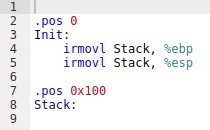
\includegraphics{img/ex_ys.png}
        \caption{Code d'un programme y86 (.ys)}
        \label{fig:ex_yo}
    \end{figure}
    
    \item \textbf{.yo} :\\
    Fichier objet contenant le code compilé à partir du .ys source.\\
    \begin{figure}[H]
        \centering
        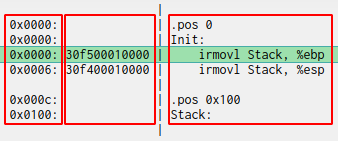
\includegraphics{img/ex_yo.png}
        \caption{fichier object (.yo) généré à partir d'un code source (.ys)}
        \label{fig:ex_yo}
    \end{figure}
    De gauche à droite, pour chaque ligne :
    \begin{enumerate}
        \item L'adresse de l'instruction
        \item Le codage de l'instruction (en hexadécimal)
        \item L'instruction même
    \end{enumerate}
    
    \item \textbf{.hcl} :\\
    Fichier décrivant le comportement du processeur face à une instruction.\\
    \begin{figure}[H]
        \centering
        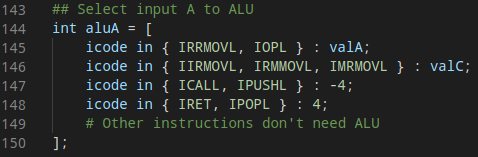
\includegraphics{img/ex_hcl.png}
        \caption{Exemple de code HCL}
        \label{fig:ex_hcl}
    \end{figure}
    Dans cet exemple, si l'instruction est IRRMOVL, alors valA sera mise dans aluA.
\end{enumerate}

\section{État de l'art}
% Etat actuel du projet

\subsection{Application web \cite{webapp-ub}}

Actuellement, la modification de quelques fichiers du simulateur web est nécessaire pour ajouter ou modifier une instruction :
\begin{itemize}
    \item \textbf{ace/mode-y86.js} qui contient les expression régulières acceptés par le compilateur.
    \item \textbf{assem.js} qui contient les fonctions nécessaire pour effectuer la conversion du code assembleur en code binaire.
    \item \textbf{general.js} qui contient les listes d'instructions avec leurs codages (\textit{icode \& ifun}).
    \item \textbf{syntax.js} qui contient une liste de toutes les syntaxes possibles.
    \item \textbf{instr.js} qui contient un tableau avec les actions de chaque instruction. Ce fichier pourra nous être utile pour récupérer l'état du processeur pour chaque étage au cas par cas). \\
\end{itemize}

Nous sommes entrain de réfléchir comment bien prendre en compte les modifications de l'utilisateur tout en gardant le sens pédagogique de l'outil avec un code flexible et modulaire.

\subsection{Application x86 (standalone)}

Cette application est le programme originel permettant de simuler un processeur y86 ainsi que sa mémoire. Elle a été créée par les professeurs R. E. Bryant et D. R. O'Hallaron, de la Carnegie Mellon University. \\
Elle propose un mode graphique (Tcl/Tk) ainsi qu'un mode textuel pour une utilisation depuis un terminal. Le comportement du processeur face aux instructions peut être modifié en utilisant le langage HCL. Ce fichier HCL est converti en fichier source C, compilé, puis lié au simulateur durant la phase d'édition de lien. Chaque modification de ce fichier nécessite donc de recompiler le simulateur (ou à minima de ré-effectuer l'édition de liens).

Plus d'informations à propos de cette application sont disponibles sur le wiki du GitLab \cite{wiki-application-y86}.

\section{Description des besoins}

Nous présenterons ci-dessous les différents besoins auxquels devra répondre l'application développée. Du fait que nous partirons très probablement d'une application déjà existante, certains besoins seront donc déjà implémentés.

Une des principales contraintes étant la facilité d'accès pour les étudiants et la portabilité, les besoins seront décrits dans l'optique du développement d'une application web.

\newpage
\subsection{Besoins fonctionnels}
% Liste des besoins
Fonctionnalités de l'application :

\begin{enumerate}
    \item \textbf{Saisie du code y86}
    \begin{enumerate}
        \item Éditeur de code y86 :\\
            Il doit respecter les contraintes suivantes :
        \begin{enumerate}
            \item Saisir du code (y86 uniquement)
            \item Afficher les numéros de lignes
            \item Colorer syntaxiquement le texte saisi
            \item Analyser statiquement le code afin d'aider à son écriture
        \end{enumerate}{}
        \begin{figure}[H]
            \centering
            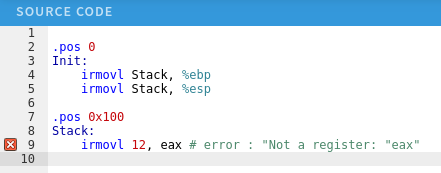
\includegraphics{img/ex_ys_erreur.png}
            \caption{Éditeur de code y86 utilisant l'analyse statique de code}
            \label{fig:ex_ys_erreur}
        \end{figure}
        
        \item Charger un fichier de code y86 \textbf{.ys} :
        \begin{enumerate}
            \item Bouton pour charger un fichier \textbf{.ys} depuis l'ordinateur de l'utilisateur. Le contenu de ce fichier est ensuite mis dans l'\textbf{éditeur de code y86} décrit précédemment.
        \end{enumerate}{}
    \end{enumerate}{}
    
    
    \item \textbf{Compilation} \\
    L'application doit être capable de générer du code objet (\textbf{.yo}) à partir du code présent dans l'\textbf{éditeur de code y86}.\\
    Les contraintes suivantes doivent être respectées :
    \begin{enumerate}
        \item un bouton permet de lancer la compilation de \textbf{ys} vers \textbf{yo}.
        \item Une fenêtre doit afficher le code \textbf{.yo} généré. L'affichage du code objet doit respecter le format des fichiers \textbf{.yo}.
        \item Si le code en entrée n'est pas valide, l'erreur de compilation doit être affichée, en rouge, dans la fenêtre précédemment citée.
    \end{enumerate}{}
    
    
    \item \textbf{Exécution} \\
    Si du code objet est présent (dans la fenêtre de compilation), l'utilisateur doit pouvoir exécuter ce code, d'une traite ou étape par étape, et doit pouvoir voir les valeurs contenues dans les registres, dans la mémoire ainsi que les drapeaux de conditions. Cela correspond à l'état de la machine. Parallèlement à ça, l'état du processeur doit aussi être visible, c'est à dire les valeurs contenues dans les différents circuits du processeur après l'exécution d'une instruction.\\ % circuit 

    Voici les besoins détaillés :
    \begin{enumerate}
            \item Affichage de l'état de la machine :
            \begin{enumerate}
                \item Les registres de \%eax à \%edi (nom, valeur en base 8, valeur en base 10)\\
                Exemple : \textbf{\%eax 0x00000100 256}
                \item Les drapeaux de condition (nom, valeur en base 10)\\
                Exemple : \textbf{SF 0}
                \item Le statut du processeur\\
                Il permet de voir le statut à proprement parlé (OK, HALT) ainsi que le compteur d'instruction, qui contient la prochaine instruction à exécuter.
            \end{enumerate}{}
            \begin{figure}[H]
                \centering
                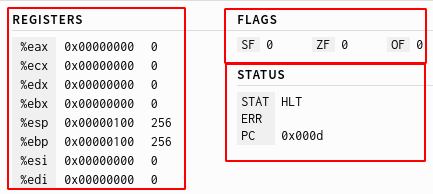
\includegraphics{img/ex_vue_registres.png}
                \caption{Registres du processeur}
                \label{fig:ex_vue_registres}
            \end{figure}
            
            \item Affichage de l'état du processeur :\\
            Affiche les différents \textit{stages} du processeur, à savoir \textbf{Fetch}, \textbf{Decode / Read}, \textbf{Execute}, \textbf{Memory} et \textbf{PC update} en séquentiel.\\
            Chaque \textit{stage} affiche une ou plusieurs valeur. Ces valeurs peuvent être de forme textuelle, ou bien numérique.\\
            Cette fenêtre est mise à jour après chaque exécution d'instruction.
            \begin{figure}[H]
                \centering
                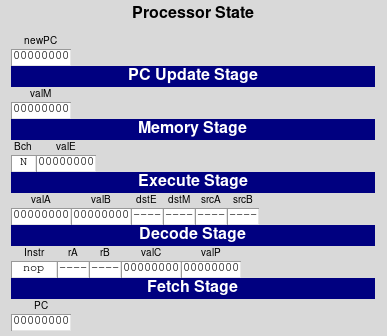
\includegraphics{img/ex_statut_proc.png}
                \caption{Vue des différents "stages" du processeur}
                \label{fig:ex_statut_proc}
            \end{figure}
    \end{enumerate}{}

    \item \textbf{Automatisation des tâches} \\
    Une fonctionnalité souhaitée est l'automatisation de certaines tâches, notamment pour les correcteurs. L'idée serait de faire des requêtes paramétrées qui retourneraient un résultat. A ce jour, la principale utilisation serait la récupération d'un dump de l'état de la machine après exécution d'un programme, avec un HCL et un IS donné, afin de voir avec quel registre / "case mémoire" le programme interagit. \\ \\
    \underline{Exemple :}\\ \textbf{wget 
    hostname?file=test.y86\&hcl=student.hcl\&conf=student.json\\\&action=memorydump\&breakline=10
    }\\

        
    \item \textbf{Personnalisation du simulateur} \\
    Le simulateur devra être personalisable. Son comportement devra pouvoir être changé de manière relativement aisée. Par exemple, on pourrait souhaiter implémenter une version \textit{pipelined} du processeur, en plus de la version \textit{sequential} de base.\\
    Un autre but pédagogique consiste à permettre aux élèves d'insérer / modifier des instructions. 
    Afin de se représenter les dépendances entre les différents modules (HCL, yas, ISA, simulateur, etc...), un diagramme disponible en annexe \ref{fig:diag_archi_modulaire} montre une potentielle esquisse d'architecture, ainsi que les dépendances entre les différents composants.
    
    \begin{enumerate}
        \item Simulateur y86 : \\
        Il s'agit du module qui exécutera les instructions contenues dans le .yo en simulant le processeur.
        \item Édition du fichier HCL : \\
        Le HCL est le code à éditer si l'on souhaite ajouter / modifier le comportement d'une instruction. Une fois le code HCL saisi, il faudra le compiler en JavaScript afin que le simulateur puisse y accéder.
    \end{enumerate}
\end{enumerate}


\subsection{Besoins non fonctionnels}
% Liste des besoins
\begin{itemize}
    \item Modularité :\\
    L’objectif à long terme est d’avoir un simulateur flexible et modulaire. De ce fait, un effort sur l’architecture devra être fait afin de permettre de rendre les choses "dynamiques". Le but est d’avoir à modifier le moins de choses possible pour ajouter / modifier un comportement.\\
    Est notamment concerné le triplet (état du processeur, InstructionSet, HCL).
    
    \item Longévité :\\
    Afin de permettre au projet de vivre dans le temps, le code devra être bien segmenté, une documentation rédigée. Ainsi qu’un cahier de maintenance (très technique) afin d’aider de potentiels successeurs à s’approprier le code et à faire évoluer l'application.
\end{itemize}
    
\subsection{Prototypage et architecture}
% Schémas de l'interface, de l'architecture que l'on mettrait en place etc..
% Tout ce qui sert à se représenter ce en quoi consistera notre travail

\section{Planification des tâches}
% El famoso diagrame de Gantt

\printbibliography

\newpage
\section{Annexes}

\begin{appendix}

\begin{figure}
    \centering
    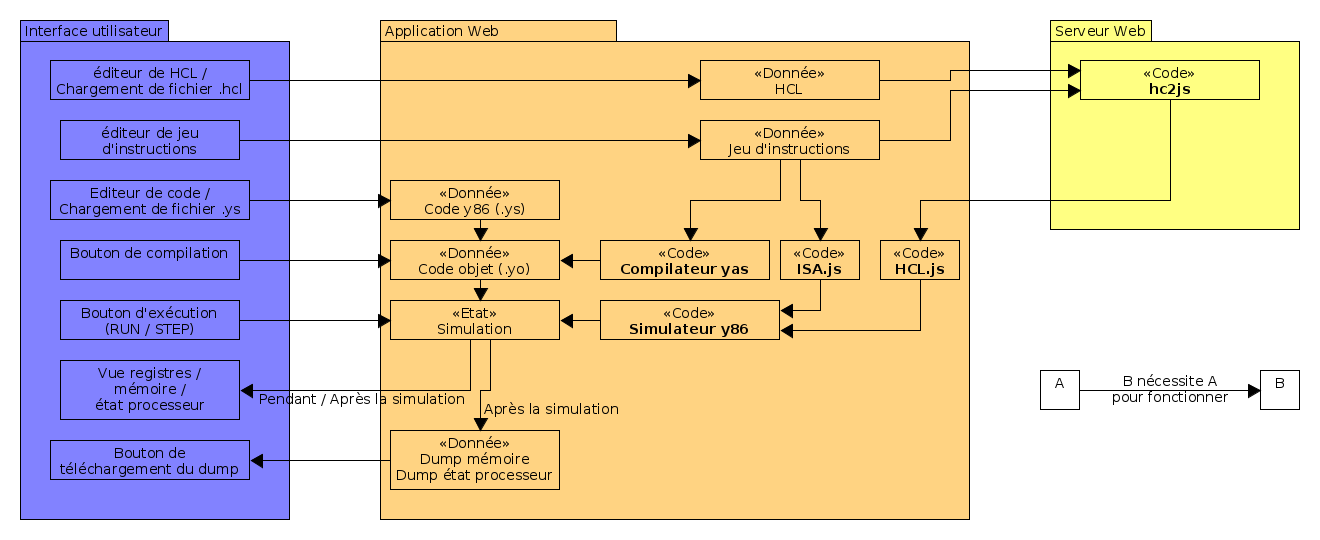
\includegraphics[width=\paperwidth, angle=270]{img/architecture_modulaire.png}
    \caption{Diagramme présentant une possible architecture pour une application web}
    \label{fig:diag_archi_modulaire}
\end{figure}

\end{appendix}

\end{document}
